\documentclass{book}
%\input{latexmacro}
\usepackage{graphicx}
\usepackage{amsmath}
\usepackage{amssymb}
\usepackage{verbatim}
\usepackage{hyperref}
\DeclareMathOperator*{\E}{\mathbb{E}}
\begin{document}
\setcounter{chapter}{3}


% special version of Chapter 4 for Louis to edit to create Python version based
% Python 3 and SimPy 3.2
% 5/24/2016
% definitions added just for this version
% Further used as a starting point by
\newtheorem{example}{Example}[chapter]
\def\ttf{\texttt{TTF}}
\def\Clock{\texttt{Clock}}
\def\Entity{\textttf{Entity}}
\def\D{\mathrm{d}}
\def\yield{\texttt{yield}}
\def\EventNotice{\texttt{EventNotice}}
%\def\Process{\texttt{Process}}
%\def\Resource{\texttt{Resource}}
\def\Level{\textbf{Level}}
\def\Store{\textbf{Store}}
\def\Monitor{\textbf{Monitor}}
\def\Tally{\textbf{Tally}}
% end special definitions

\chapter{Simulation Programming with Python 3 and SimPy 3}
\label{ch:pythonsim}
\index{Python}
\index{SimPy}

This chapter shows how simulations of some of the examples in
Chap. 3  can be programmed using Python 3.x and the SimPy 3 simulation library\cite{SimPy2016}\footnote{by Louis Luangkesorn <louis.luangkesorn@gmail.com>. This is intended to be an appendix to \cite{Nelson2013} which can be obtained at \url{http://users.iems.northwestern.edu/~nelsonb/IEMS435/}.  These language supplements replace Chapter 4 in that book.}.
The goals of the chapter are to introduce SimPy, and to hint at the experiment design and analysis issues that will be covered in later chapters. %Chap. 3 {%~\ref{ch:examples}}
While this chapter will generally follow the flow of Chap. 4 from the main text, it will use the conventions and patterns consistent with process-based simulations with the SimPy library instead of the event-scheduling approach of VBASim. 

\section{Simulation overview}

As an example of a simulation using Python we use the time to failure example described in Chapter 2.  The code is in Figure \ref{fig:ttfhelper}.

\begin{figure}[tbp]
\begin{minipage}[t]{6in}\small
\verbatiminput{TTFhelper.py}
\end{minipage}
\caption{Time to failure functions.}
\label{fig:ttfhelper}
\end{figure}

In a Python program, we start with importing libraries. In this case we import the \texttt{random} library to generate random numbers.  

Next, we will define global variables. In keeping with good software practice we don't create variables with true global scope, instead we create a globally available class \textbf{T} with members being the required global values.
These values include initialization values for state and clock variables.

For the simulation itself, we will define the processes that will occur during the simulation. There are two process functions: \texttt{Failure()} and \texttt{Repair()}.
Each of them change the state variable tracking the number of working stations, \texttt{T.S}, schedule the next failure or repair event, and update the simulation performance measure \texttt{T.Area}.
Finally each process returns the updated state of the system.

The \texttt{TimerFunc()} function manages the simulation clock.  It determines which is the next event 	and advances the simulation clock to the next event.  

\begin{figure}[tbp]
\begin{minipage}[t]{6in}\small
\verbatiminput{TTF.py}
\end{minipage}
\caption{Time to failure main simulation.}
\label{fig:ttf}
\end{figure}

The function \texttt{TTF(aseed)} in Figure \ref{fig:ttf} is the main function of the simulation.
It takes one parameter, the random number seed \texttt{aseed}, which ensures reproducability of the results.
It initializes all state and clock variables, then sets in motion initial processes.  It continues until the stopping condition is met.  In \texttt{TTF}, the stopping condition is when both machines are out of operations (failed).	
Finally, it processes statistics and performs any reporting required.
Figure \ref{fig:ttfoutput} shows the output of the simulation.  While normally you would not print out the status after every event, at times it may be useful to do so to help confirm that the simulation program is behaving as intended.

\begin{figure}
\begin{minipage}[t]{6in}\small
\begin{verbatim}
We are beginning the TTF simulation!
At time
0
we have 2 machines operating
There is a failure occurring at time 4
At time
4
we have 1 machines operating
There is a failure occurring at time 5
There are no machines left!
The time of failure is 5
The average number of components was
1.8
\end{verbatim}
\end{minipage}
\caption{Time to failure output}
\label{fig:ttfoutput}
\end{figure}

In this simple simulation, the program manages many details such as the simulation clock and the state of the system. In practice, the simulation library that you use will manage the simulation clock and track the state of the system. One such library is the SimPy simulation library in Python.

\section{SimPy Overview}
\label{sec:SimPy.overview}


SimPy is a process-based discrete-event simulation framework based on standard python.
SimPy is built upon a special type of Python function called \textbf{generators} \footnote{\url{https://wiki.python.org/moin/Generators}}.
When a generator is called, the body of the function does not execute, rather, it returns an iterator object that wraps the body, local variables, and current point of execution (initially the start of the function).
This iterator then runs the function body up to the \texttt{yield} statement, then returns the result of the following expression.
This generator will be used to represent recurrent processes, such as entities in an arrival stream, as well as the steps in the process that an entity experiences as it moves through the system.

Being \textit{process-based} means that the simulation is viewed in terms of the individual entities involved, where the entities are described in terms of the path experienced by the entitity as it moves through the system. This is in contrast to the \textit{event-scheduling} approach used in VBASim which explicitly adds scheduled events into the the simulation next event list, then each event triggers future events.

In a SimPy simulation model, the behavior of all entities is modeled with \textit{processes}.  All processes in the same model exist in an \textit{environment}.  Entities intereact with the environment and each other through \textit{events}.

 SimPy provides the modeler with components of a simulation model including processes, for active components like customers, messages, and vehicles, and resources, for passive components that form limited capacity congestion points like servers, checkout counters, and tunnels. It also allows for monitor variables to aid in gathering statistics. Random variates are provided by the standard Python random module or other random number generators.  Beginning with SimPy 3.0.1, SimPy runs on Python 3.  There is also a port of SimPy for use on the .NET called Sim\#\footnote{\url{https://github.com/abeham/SimSharp}}.  Full documentation can be found at the SimPy website\footnote{\url{https://simpy.readthedocs.io/en/latest/index.html}}.  This chapter and its companion code will use Python 3.x and SimPy 3.x. \footnote{ An earlier version of this chapter were written for Python 2.7.x and SimPy 2.3 and is still available at the textbook website \url{http://users.iems.northwestern.edu/~nelsonb/IEMS435/code.htm}}.

As SimPy is a library within a full featured programming language, Python and its associated libraries provide the data collection, data analysis, and statistics and reporting capabilities needed for analyzing data and simulation output\cite{Scipy2001}.
Python libraries can also be used to access databases with simulation parameters or store simulation results.\footnote{A list of the core scientific libraries that make up the scientific python stack can be found at \url{https://www.scipy.org/about.html}.}
The simulation model can also be part of an analysis pipeline, where results of other analysis can be used as inputs into the simulation model, and the results can be used in other analysis.

This chapter will use SimPy along with the following libraries:

\begin{enumerate}
\item Numpy\footnote{http://www.numpy.org} is the fundamental 	package for scientific computing with Python. It includes high-performance arrays, tools for integrating C/C++ and Fortran code, linear algebra, and random number generation capabilities. These are often used by other packages as computational building blocks.
\item Scipy\footnote{http://www.scipy.org} is a collection of scientific libraries that are built on Numpy.  Of particular importance are the scipy.stats library, which includes random variate generation.
\item Pandas\footnote{http://pandas.pydata.org/} provides high performance data structures and data analysis tools.
\item Matplotlib\footnote{http://matplotlib.org/} is a flexible plotting library. Pandas provides a simplified interface for some standard plots.
\item Statsmodels\footnote{http://statsmodels.sourceforge.net/} provides a range of statistical analysis methods, including a range of statistical tests, variations on linear regression models, and time series analysis.
\end{enumerate}

The easiest way to install Python along with its scientific libraries (including SimPy) is to install a scientifically oriented distribution, such as Enthought Canopy\footnote{http://www.enthought.com/products/canopy/} or Anaconda Python distribution \footnote{https://www.anaconda.com/} for Windows, Mac OS X, or Linux.
If you are installing using a standard Python distribution, you can install SimPy by using \texttt{pip}.

\begin{verbatim}
pip install simpy
\end{verbatim}

Users of Anaconda can use the \texttt{conda} package manager.

\begin{verbatim}
conda install -c mutirri simpy
\end{verbatim}

The other required libraries can be installed in a similar manner.  See the specific library webpages for more information.

This chapter will assume that you have the Numpy, Scipy, Pandas, Matplotlib, and Statsmodels libraries installed.

In this simple car example (Figure \ref{fig:simpleparking}), the car alternates between parking and driving for a specific duration.

First, the \texttt{simpy} library is loaded.  Other libraries that may be needed include Matplotlib or Scipy.

Next, the process function defines the path an entity takes within the simulation. In this case, it is a car that takes alternates between parking and taking trips on a regular schedule.  
The duration of each activity is indicated by the \texttt{yield} statement.  The \texttt{env.timeout()} function indicates how long the process pauses before continuing to the next event.  In this simulation, the process repeats continuously until the stopping condition, indicated by \texttt{env.run(until=15)}, is reached.

The main program creates the \texttt{simpy.Environment()} in which the simulation takes place.
It adds all processes and resources that are part of the simulation using the \texttt{process()} function or the \texttt{resource()} function to be discussed later.
Then the \texttt{run()} function starts all processes until all processes complete or until the stopping condition, \texttt{until=15}, is reached.

\begin{figure}[tbp]
\begin{minipage}[t]{6in}\small
\verbatiminput{simplecar.py}
\end{minipage}
\caption{Simple parking example.}
\label{fig:simpleparking}
\end{figure}

\subsection{Random numbers}

Discrete event simulation makes heavy use of random numbers.
There are two implementations of random-variate generations functions generally used within Python, \texttt{random} from the Python Standard Library and the random variate generators in the \texttt{scipy.stats} module. The \texttt{scipy.stats} module is generally more flexible and faster. The \texttt{random} module is used when it is important for the code to be easy to read by a non-programmer or when the \texttt{scipy.stats} module is unavailable (e.g. you are using Jython or Iron Python or a computer where you only have the standard library).

The \texttt{random} module of the Python Standard Library is based on the Mersenne Twister as the core generator.
This generator is extensively tested and produces 53-bit precision floats and a period of $2^{19937}-1$.
Some distributions included in the the \texttt{random} module include uniform, triangular, Beta, Exponential, Gamma, Gaussian, Normal, Lognormal, and Weibull distributions.

The basic use of random variate generators in the \texttt{random} module is as follows:

\begin{enumerate}
	\item Load the \texttt{random} module:  \texttt{import random}
	\item Instantiate a generator:   \texttt{g = random.Random()}
	\item Set the seed:  \texttt{g.seed(1234)}
	\item Draw a random variate:
	\begin{itemize}
		\item A random value from 0 to 1:  \texttt{g.random()}
		\item A random value (float) from a to b:  \texttt{g.uniform(a,b)}
		\item A random integer from a to b (inclusive): \texttt{g.randint(a, b)}
		\item A random sample of $k$ items from list $population$:  \texttt{g.sample(population, k)}
	\end{itemize}
\end{enumerate}

The \texttt{scipy} module includes a larger list of random variate generators including over 80 continuous and 10 discrete random variable distributions.
For each distribution, a number of functions are available including the following:

\begin{itemize}
    \item \texttt{rvs}: Random Variates generator,
    \item \texttt{pdf}: Probability Density Function,
    \item \texttt{cdf}: Cumulative Distribution Function,
    \item \texttt{stats}: Return mean, variance, (Fisher's) skew, or (Fisher's) kurtosis,
\end{itemize}

As over 80 distributions are included, the parameters of the distributions are in a standardized form, with the parameters being the location, scale and shape of the distribution.
The module documentation and a probability reference may be consulted to relate the parameters to those that you may be more familiar with.

The basic use of Scipy random number generators is as follows.

\begin{enumerate}
	\item Load the Scipy module.
		\begin{verbatim}
			import scipy as sp
		\end{verbatim}
	\item Set the random number seed.  Scipy uses the Numpy random number generators so the Numpy random.seed function should be used:  \texttt{sp.random.seed(1234)}
	\item Instantiate the generator\footnote{this method is referred to in the Scipy documentation as \em{freezing a distribution}.}.  Some examples:
		\begin{itemize}
			\item  Normal with mean 10 and standard deviation 4:  \\
					\texttt{norm1 = sp.stats.norm(loc = 10, scale = 4)}
			\item  Uniform from 0 to 10: \\
					\texttt{unif1 = sp.stats.uniform(loc = 0, scale = 10)}
			\item  Exponential with mean 1: \\
					 \texttt{expo1 = sp.stats.expon(scale = 1.0)}
		\end{itemize}
	\item  Generate a random value:  \texttt{norm1.rvs()}.
\end{enumerate}

\section{Simpy introduction}

In SimPy simulations, all active components are modeled with processes. All processes in a single simulation exist in an environment and interact with each other through events.

We will use the car wash simulation in Figure \ref{fig:carwash} adapted from the SimPy documentation as an example in exploring SimPy.

\begin{figure}[tbp]
\begin{minipage}[t]{6in}\small
\verbatiminput{carwash_monitor.py}
\end{minipage}
\caption{Car wash simulation.}
\label{fig:carwash}
\end{figure}

The Car wash simulation program imports the SimPy, scipy, random, and pandas libraries; defines a process function, and adds monitoring capability to the car wash resource class.
The main portion of the simulation declares the simulation environment, sets up the car wash as a monitored resource, then generates a series of cars as processes that go through the resource.  
The simulation then calculates statistics on resource use, using the monitoring capability added to the carwash resource as shown in Figure \ref{fig:carwashmonitor}. 

\begin{figure}[tbp]
\begin{minipage}[t]{6in}\small
\verbatiminput{MonitoredResource.py}
\end{minipage}
\caption{Monitored Resource class for the car wash simulation.}
\label{fig:carwashmonitor}
\end{figure}


\subsection{Processes}

Processes are described using generators.  Generally, a process method would be a method of a class. In a simple simulation it may be a simple process function.  
Within SimPy, the \texttt{yield} statements are used to define the event scheduling.
This is used for a process to either do something to itself (e.g. the next car arrives); to request a resource, such as requesting a server; to release a resource, such as a server that is no longer needed; or to wait for another event.

In the carwash simulation, the \texttt{car} function defines the process.  The \texttt{yield env.timeout()} statements introduce delays due to the the car driving to the car wash and the duration of the car wash itself.
The \texttt{yield req} requests the car wash resource.  If a car wash is available, it would claim the resource for the duration specified in the \texttt{yield env.timeout()} statement that follows.  If no car wash was available, the car would enter the queue and wait for a car wash to become available.

\subsection{Resources}

Sometimes, events require a resource with a limited capacity. Resources represent a limiting element in the system where entities must line up and in order to use them.

SimPy defines three categories of resources:

\begin{itemize}
\item Resources - Resources that can be used by a limited number of process as a time.
\item Containers - Resources the production and consumption of a homogeneous, undifferentitated bulk item.
\item Stores - Resources that allow the production and consumption of objects.  Unlike containers, a Store can contain multiple types of objects.
\end{itemize}

For each type of resource, you can specify the queue discipline (usually first in, first out), requesting processes can have different priority levels, and it is possible to specify preemption.\footnote{https://simpy.readthedocs.io/en/latest/topical\_guides/resources.html}

To declare a resource, you declare it as part of an environment, and you state its capacity. If you do not state its capacity, the default capacity is 1.

\begin{verbatim}
import simpy
env = simpy.Environment()
carwash = MonitoredResource(env, capacity=C.NUM_MACHINES)
\end{verbatim}

To utilize the resource, a process must request the resource.  
To do this, when the process is defined, it should be passed the resource, then request the resource.  When the request is filled, the process will \texttt{timeout} for the period of time that it occupies the resource, at which point it will release the resource as it continues along its path through the system.

\begin{verbatim}
def car(env, name, cw, driving_time, wash_duration):
    yield env.timeout(driving_time)
    with cw.request() as req:
        yield req
        yield env.timeout(wash_duration)
\end{verbatim}

There are two ways of requesting a resource.  The first is as shown in the above example which uses the \texttt{with} statement to make a \texttt{request}.  
The second way to request a resource is to use a \texttt{request} function without the \texttt{with} statement. If you use the second method, you need to use the \texttt{release} function when the process is done with the resource to free the resource for another process.

\subsubsection{Monitoring a resource}

One common reason for developing a simulation is to determine the impact of a change in the system on resource use or delays at a resource experienced by customers.
To do this, the simulation must collect data on events in the simulation. Some things that need to be considered include:

\begin{itemize}
	\item Are you interested in monitoring processes (the experience of entities moving through your system)?
	\item Are you interested in resource use?
	\item Do you want to collect data at key events?
	\item Are you collecting data at regular time intervals?
\end{itemize}

Because SimPy is a simulation library of a general purpose programming language, a data collection feature can be added to any process or resource and it can be stored in any data structure (list, panda) or persistant data location (e.g. file or data base) based on the future analysis needs. 


In the carwash simulation, the \texttt{MonitoredResource} class collects data by creating a data collection list (\texttt{self.data=[]}, then appending data as event occur that involve that resource. In this case, these are the \texttt{request()} and \texttt{release()} functions.  Both of these functions have a line that adds data to the data collection list including the timestamp, the number of stations currently in operation, and the number of cars waiting in the carwash queue.

\texttt{self.data.append((self.\_env.now, self.count, len(self.queue)))}

At the end of the simulation, the \texttt{updatestats()} function takes the list of time stamps, the converts it into a \texttt{pandas} data structure for processing.  The \texttt{updatestats()} function also processes the data into elapsed time, which is more useful for calculating time average statistics as done in the \texttt{timeAverage()} function.

These statistical functions are then called at the end of the simulation for reporting results.

Note that this monitored resource class is very useful capability for specific performance measures of interest \footnote{More discussion on adding monitors in Simpy can be found at \url{https://simpy.readthedocs.io/en/latest/topical_guides/monitoring.html}.}.

\subsection{Running the simulation}

To run the simulation, after we create an instance of \texttt{Environment}, we add any processes to the environment.  Then we can use the \texttt{run} function to start all processes until they have completed or a stopping condition is reached.
In the case of the car wash, it runs until \texttt{C.NUM\_CARS} cars have gone through the car wash.

\section{Simulating the $M(t)/M/\infty$ Queue}
\label{sec:sim.mminf}

Here we consider the parking lot example of Sect.~3.1, %\ref{sec:mminf},
which is a queueing system with time-varying car arrival rate, exponentially
distributed parking time and an infinite number of parking spaces.

A SimPy simulation generally consists of import of modules, defining processes and resources, defining parameters, a main program declaring, and finally reporting.

At the top of the program are imports of libraries used.  (Fig.~\ref{fig:parking.import}).
First we import libraries from the Python standard library such as \texttt{math} and \texttt{random}.
Next, we import in other modules and modules we may have written ourselves.
While you could also import directly into the global namespace using the construct \texttt{from SimPy.Simulation import *}, instead of \texttt{import SimPy.Simulation as Sim}, this is discouraged as there is a potential of naming conflicts if two modules happened to include functions or classes with the same name.

PARKING SIMULATION NOT WORKING CORRECTLY
\begin{figure}[tbp]
\begin{minipage}[t]{6in}\small

\verbatiminput{parking_simpy3.py}
\end{minipage}
\caption{Parking simulation example.}
\label{fig:parking.import}
\end{figure}


Next are two components, the cars and the source of the cars. (Fig.~\ref{fig:parking.components})
Both of these are classes that subclass from \textbf{Sim.Process}.
The class \texttt{Arrival} generates the arriving cars using the \texttt{generate} method.
The mean arrival rate is a function based on the time during the day.
Then the actual interarrival time is drawn from an exponential distribution.


Within the \texttt{Car} object, the \texttt{yield env.timeout(timeparking)} line is used to represent the time that the car remains in the parking lot.  To look at this line more closely

\begin{enumerate}
	\item \texttt{yield}: a Python keyword that returns a generator.  In this case, it calls the function that follows in a computationally efficient manner.
	\item \texttt{env.timeout()}:  This causes a process to wait while the object is performing an action. In this case it is the car occupying a resource (parking spot).
	\item \texttt{env}:  A reference to the current simulation.  In this case it means the currently created Car should wait for a period of time within the simulation.
	\item \texttt{timeParking}:  The time that the Car should wait.  This was created by the Arrival generator and passed to the Car object when it was created.
\end{enumerate}


In this case, since the purpose of the simulation is to determine demand for parking spaces, we assume there are unlimited spaces and we count the number of cars in the parking lot at any point in time.

In SimPy, resources such as parking spaces are represented by Resources.
There are three types of resources.

\begin{itemize}
	\item A \textbf{Resource} is something whose units are required by a \textbf{Process}.  When a \textbf{Process} is done with a unit of the \textbf{Resource} it releases the unit for another \textbf{Process} to use.  A \textbf{Process} that requires a unit of Resource when all units are busy with other Processes can join a queue and wait for the next unit to be available.
	\item A \textbf{Level} is homogeneous undifferentiated material that can be produced or consumed by a \textbf{Process}.  An example of a level is gasoline in a tank at a gas station.
	\item A \textbf{Store} models the production or consumption of specific items of any type.  An example would be a storeroom that holds a variety of surgical supplies,
\end{itemize}

Global declarations are in the top of the file in the class \textbf{G}.  While Python allows these to be in the global namespace, it is preferred that these be put into a class created for the purpose as shown here.

The main simulation class is shown in Fig.~\ref{fig:parking.main}.
The simulation class \texttt{Parkingsim} is a subclass of \textbf{Sim.Simulation}.
While it can have other functions, the central function is the \texttt{run(self)} function.
Note that the first argument of a member function of a class is \texttt{self}, indicating that the function has access to the other functions and variables of the class.
The \texttt{run} function takes one argument, the random number \texttt{seed}.
\texttt{Sim.initialize()} sets all Monitors and the simulation clock.
Then processes and resources are created.  In this simulation there is one process, the generation of arriving cars in \texttt{Arrival}.  Note that at this point, there are no \texttt{Car}'s, as the \texttt{Arrival} process will create the cars.
This simulation does not have any resources; but if, for example, the parking lot had a limited capacity of 20 spaces, it could have been created here by:

NEED A DISCUSSION OF MONITORED RESOURCES HERE

\texttt{self.parkinglot = Sim.Resource(capacity = 20, name='Parking lot', unitName='Space', monitored=True, sim=self)}



This creates the parking lot with 20 spaces.  By default, resources are a FIFO, non-priority queue with no preemption.
In addition to the capacity of the Resource (number of servers), there are two queues (lists) associated with the resource.  First is the \texttt{activeQ}, which is the list of process objects currently using the resource.  Second is the \texttt{waitQ}, which is the number of processes that have requested but have not yet received a unit of the resource.  If when creating the resource the option \texttt{monitored=True} is set, then a \textbf{Monitor} is created for each queue, and statistics can be collected on resource use and the wait queue for further analysis.
The last option is \texttt{sim=self}, which declares that the Process or Resource is part of the simulation defined in the current class derived from \textbf{Sim.Simulation}.  If the simulation was defined in the global namespace (not inside of a \textbf{class}), then this option would not be needed.

\begin{figure}[tbp]
\begin{minipage}[t]{6in}\small
REMOVE THIS
\end{minipage}
\caption{Main Simulation.}
\label{fig:parking.main}
\end{figure}

After Processes and Resources are created, any additional Monitors are created here.  Note that Processes, Resources, and Monitors are created using \texttt{self.} constructs.  This classifies the object as part of the class, and not only local to the \texttt{run()} function.  Other classes and methods that are part of this simulation (declared using \texttt{sim = self}) can refer to any object created here using \texttt{self.sim.objectname}.  This includes Monitors as well as variables that need to be updated from anywhere in the simulation.  For example, the variable \texttt{self.parkedcars} can be updated from the \texttt{Car} class in Fig.~\ref{fig:parking.components} using \texttt{self.sim.parkedcars}.

Following the main simulation class, the class is instantiated using \texttt{parkinglot = Parkingsim()}, then the simulation is run using \texttt{parkinglot.run(seedvalue)}.
One advantage of using a simulation class and object is that the monitors created in the simulation are available to the object instance \texttt{parkinglot} after the simulation is run.
If the simulation is run from within the Python command line or the IPython notebook\footnote{http://ipython.org}, this allows for interactive exploration of the simulation results.
For example, the monitor \texttt{parking} monitors the number of cars that are in the parking lot by time.  So a graph can be plotted that tracks the number of cars over the course of the 24 hour day. (Fig.~\ref{fig:parking.plotting})  The steps are:

\begin{enumerate}
	\item Load matplot lib (Fig.~\ref{fig:parking.import}) \texttt{import matplotlib.pyplot as plt}
	\item Set figure size \texttt{plt.figure(figsize=(5.5,4))};
	\item Define the plot. Note the use of the attributes of the monitor \texttt{parking}.
      {\texttt{plt.plot(parkinglot.parking.tseries(),
            parkinglot.parking.yseries())}}
	\item Set labels and other options
\end{enumerate}

\begin{figure}[tbp]
\begin{minipage}[t]{6in}\small
\begin{verbatim}
plt.figure(figsize=(5.5,4))
plt.plot(parkinglot.parking.tseries(),parkinglot.parking.yseries())
plt.xlabel('Time')
plt.ylabel('Number of cars')
plt.xlim(0, 24)
\end{verbatim}
\end{minipage}
\caption{Plotting results.}
\label{fig:parking.plotting}
\end{figure}

This results in the plot in Fig.~\ref{fig:parkedcars.plot}.

\begin{figure}[tbp]
\centerline{\includegraphics[width=4in]{figures/parkedcars}}
\caption{Number of parked cars over time.}
\label{fig:parkedcars.plot}
\end{figure}

To make inferences or conclusions based on the simulation, it is necessary to run the simulation many replications.  So to find the daily average of the number of cars, we can run the simulation over 1000 days and look at the average and maximum parking over that period.  Fig.~\ref{fig:parking.replications} shows how to do this using a \texttt{for} loop.\footnote{The Python scientific libraries include provisions for working with multi-core processors that this chapter will not utilize.}
For each replication, initialize the \texttt{parkinglot} instance of the simulation object, then \texttt{run} using a new random number seed.
Then, \texttt{append} the simulation results to a list object that was initialized using \texttt{parkingdemand = []}.  Note that any object can be appended to a list.  In this case the monitor \texttt{parking} for each simulation run was saved to the list \texttt{parkingdemand}.


\begin{figure}[tbp]
\begin{minipage}[t]{6in}\small
\begin{verbatim}
initialseed = 4321
parkingdemand = []
daysrep = 1000
for i in range(daysrep):
    parkinglot.initialize()
    parkinglot.run(initialseed + i)
    parkingdemand.append(parkinglot.parking)
\end{verbatim}
\end{minipage}
\caption{1000 replications}
\label{fig:parking.replications}
\end{figure}

From this list of simulation monitor results, one can then extract a particular data element, then calculate statistics from it.  So, for each simulation monitor saved to \texttt{parkingdemand}, the time average number of cars in the lot is given by \texttt{parkingdemand[i].timeAverage()}.  So, to have a list of the time average number of cars for each replication, we can use the list comprehension

\texttt{[parkingdemand[i].timeAverage() for i in range(daysrep)]}.

The construct \texttt{[function(i) for i in range(datasetlength)]} is known as a list comprehension.  It is a compact method for stating:

\begin{verbatim}
for i in range(datasetlength):
	function(i)
\end{verbatim}

In addition to being more compact, this construct is used often in data analysis because it can be relatively easily parallelized if the computing facilities are available.
The resulting list can then be analyzed through visualization or statistics.  In Fig.~\ref{fig:parking.average.cdfplot} there is the resulting cumulative histogram.

\begin{figure}[tbp]
\begin{minipage}[t]{6in}\small
\begin{verbatim}
averagedailyparking = [parkingdemand[i].timeAverage() for
                i in range(daysrep)]
plt.hist(averagedailyparking, bins=25, cumulative = True,
                label = 'Average number of cars during day')
plt.xlabel('Average number of cars in day')
plt.ylabel('Days (cumulative)')
\end{verbatim}
\end{minipage}
\caption{1000 replications}
\label{fig:parking.averageparking}
\end{figure}

\begin{figure}[tbp]
\centerline{\includegraphics[width=4in]{figures/averagecars}}
\caption{Cumulative histogram of average number of parked cars.}
\label{fig:parking.average.cdfplot}
\end{figure}

Fig.~\ref{fig:parking.maximumparking} shows a standard histogram of the maximum number of cars parked in a given simulation day, indicated by the option \texttt{cumulative=False}.  The corresponding plot is in Fig.~\ref{fig:parking.maximum.cdfplot}.

\begin{figure}[tbp]
\begin{minipage}[t]{6in}\small
\begin{verbatim}
maxparkingdailyparking = [max(parkingdemand[i].yseries())
                for i in range(daysrep)]
plt.hist(maxparkingdailyparking, bins=25, cumulative = False)
plt.xlabel('Maximum number of cars')
plt.ylabel('Days (cumulative)')
\end{verbatim}
\end{minipage}
\caption{Maximum number of cars parked in a day.}
\label{fig:parking.maximumparking}
\end{figure}

\begin{figure}[tbp]
\centerline{\includegraphics[width=4in]{figures/maximumcars}}
\caption{Histogram of maximum number of parked cars.}
\label{fig:parking.maximum.cdfplot}
\end{figure}

We think that the distribution of the average number of cars in the lot on any given day follows a normal distribution.  We can test this using the the \texttt{sp.stats.normaltest} function. (Figure \ref{fig:parking.testnormalprob})
In addition, we can plot a normal probability plot using the \texttt{sp.stats.statsplot} function.  Figure \ref{fig:parking.statsplot} shows a normal probability plot that is consistant with a hypothesis that the average number of cars in a day follows a normal distribution.

\begin{figure}[tbp]
\begin{minipage}[t]{6in}\small
\begin{verbatim}
testvalue, pvalue = sp.stats.normaltest(averagedailyparking)
print(pvalue)

0.761955484599
\end{verbatim}
\end{minipage}
\caption{Test for normality for average cars parked.}
\label{fig:parking.testnormalprob}
\end{figure}

\begin{figure}[tbp]
\centerline{\includegraphics[width=4in]{figures/avgparkingstatsplot}}
\caption{Normal probability plot of average cars parked in a day generated by \texttt{scipy.stats.statsplot()}.}
\label{fig:parking.statsplot}
\end{figure}


\subsection{Issues and Extensions}
\label{sec:sim.mminf.issues}

\begin{enumerate}

\item The $M(t)/M/\infty$ simulation presented here simulates $24$
hours of parking lot operation, and treats each $24$-hour period
as as independent replication starting with an empty garage. This only
makes sense if the garage is emptied each day, for instance if the
mall closes at night. Is the assumed arrival rate $\lambda(t)$
appropriate for a mall that closes at night?

\item Suppose that the parking lot serves a facility that is
actually in operation $24$ hours a day, seven days per week (that is,
all the time). How should the simulation be initialized, and how long
should the run length be in this case?

\item How could the simulation be initialized so that there are $100$
cars in the parking lot at time $0$?

\item When this example was introduced in Sect.~3.1 %\ref{sec:mminf}
, it was suggested that we size the garage based on the (Poisson)
distribution of the number of cars in the garage at the point in time
when the mean number in the garage was maximum. Is that what we did,
empirically, here? If not, how is the quantity we estimated by
simulation related to the suggestion in Sect.~3.1%\ref{sec:mminf}
(for instance, will the simulation tend to suggest a bigger or smaller
garage than the analytical solution in Sect.~3.1%\ref{sec:mminf})?

\item One reason that this
simulation executes quite slowly when $\lambda(t) = 1000 +
100\sin(\pi t/12)$ is that the thinning method we used is very
inefficient (lots of possible arrivals are rejected). Speculate about
ways to make it faster.

\item For stochastic processes experts: Another reason that the
simulation is slow when $\lambda(t) = 1000 + 100\sin(\pi t/12)$ is
that there can be $1000$ or more pending departure events in the event list at any time,
which means that scheduling a new event in
chronological order involves a slow search. However, it is possible
to exploit the memoryless property of the exponential distribution of
parking time to create an equivalent simulation that has only two
pending events (the next car arrival and next car departure) at any
point in time. Describe how to do this.

\end{enumerate}


\section{Simulating the $M/G/1$ Queue}
\label{sec:sim.mg1}

Here we consider the hospital example of Sect.~3.2, %\ref{sec:mg1}
a queueing system with Poisson arrival process, some (as yet
unspecified) service-time distribution, and a single server (either a
receptionist or an electronic kiosk). In other words, an $M/G/1$
queue.\index{$M/G/1$ queue} Patient waiting time is the key system
performance measure, and the long-run average waiting time in
particular.

Recall that Lindley's Equation~(3.3) % (\ref{eq:lindley})
provides a shortcut
way to simulate  successive customer waiting times:\index{Lindley's Equation}
\begin{eqnarray*}
Y_0 &=& 0 \qquad X_0 = 0 \\
Y_i &=& \max\{0, Y_{i-1} + X_{i-1} - A_i\},\ i=1,2,\ldots
\end{eqnarray*}
where $Y_i$ is the $i$th customer's waiting time, $X_i$ is that
customer's service time, and $A_i$ is the interarrival time between
customers $i-1$ and $i$. Lindley's equation avoids the need for an
event-based simulation, but is limited in what it produces (how would
you track the time-average number of customers in the queue?). In
this section we will describe both recursion-based and event-based
simulations of this queue, starting with the recursion.

\subsection{Lindley Simulation of the $M/G/1$ Queue}
\label{sec:sim.mg1.lindley}

To be specific, suppose that the mean time between arrivals is $1$
minute, with the distribution being exponential, and the mean time to use
the kiosk is $0.8$ minutes ($48$ seconds), with the distribution
being an Erlang-$3$.\index{Erlang distribution} An Erlang-$p$ is the
sum of $p$ i.i.d.\ exponentially distributed random variables, so an
Erlang-$3$ with mean $0.8$ is the sum of $3$ exponentially
distributed random variables each with mean $0.8/3$.

In Sect.~3.2 %\ref{sec:mg1}
we noted that the waiting-time
random variables $Y_1, Y_2, \ldots$ converge in distribution to a
random-variable $Y$, and it is $\mu = \E(Y)$ that we will use to
summarize the performance of the queueing system. We also noted that
$\bar{Y}(m) = m^{-1}\sum_{i=1}^m Y_i$ converges with probability $1$
to $\mu$ as the number of customers simulated $m$ goes to infinity.

All of this suggests that we make a very long simulation run (large
$m$) and estimate $\mu$ by the average of the observed waiting times
$Y_1, Y_2, \ldots, Y_m$. But this is not what we will do, and here is
why: Any $m$ we pick is not $\infty$, so the waiting times early in
the run---which will tend to be smaller than $\mu$ because
the queue starts empty---will likely pull $\bar{Y}(m)$ down. To
reduce this effect, we will let the simulation generate waiting times
for a while (say $d$ of them) before starting to actually include
them in our average. We will still make $m$ large, but our average
will only include the last $m-d$ waiting times. That is, we will use as
our estimator the truncated average \index{truncated average}
\begin{equation}
\label{eq:truncated.average}
\bar{Y}(m,d) = \frac{1}{m-d}\sum_{i=d+1}^m Y_i .
\end{equation}
In addition, we will not make a single run of $m$ customers, but
instead will make
$n$ replications. This yields $n$ i.i.d.\ averages $\bar{Y}_1(m,d),
\bar{Y}_2(m,d),
\ldots, \bar{Y}_{n}(m,d)$ to which we can apply standard statistical
analysis. This avoids the need to directly estimate the asymptotic
variance $\gamma^2$, a topic we defer to later chapters.

\begin{figure}[tbp]
\verbatiminput{hospitallindsey	.py}
\caption{Simulation of the $M/G/1$ queue using Lindley's equation\label{fig:hospital.lindley}.}
\end{figure}

Figure~\ref{fig:hospital.lindley} shows a Python simulation of the
$M/G/1$ queue using Lindley's equation. In this simulation
$m=55{,}000$ customers, we discard the first $d=5000$ of them, and
make $n=10$ replications.

The ten replication averages can be then individually written to an comma separated value (csv)
file named ``lindley.csv'' (Fig.~\ref{fig:hospital.lindleyout}) and also printed out to the screen with the mean and standard deviation as in Table~\ref{tab:lindley.results}.


Notice that the average waiting time
is a bit over $2$ minutes, and that Python, like all programming
languages, could display a very large number of output digits. How many
are really meaningful? A confidence interval is one way to provide an
answer.

\begin{table}[tbp]
\caption{Ten replications of the $M/G/1$ queue using Lindley's
equation.}
\label{tab:hospital.lindleyout}
\begin{center}
\begin{tabular}{cc}\hline
replication&$\bar{Y}(55000, 5000)$ \\\hline
1 & 2.0417\\
2 & 1.9358 \\
3 & 1.9926 \\
4 & 1.5551 \\
5 & 2.2140\\
6 & 2.1115 \\
7 & 2.0076 \\
8 & 1.9956 \\
9 & 1.6536 \\
10 & 2.8417 \\ \hline
average & 2.0349 \\
std dev & 0.3284\\ \hline
\end{tabular}
\end{center}
\end{table}

Since the across-replication averages are i.i.d., and since each
across-replication average is itself the within-replication average
of a large number of individual waiting times ($50{,}000$ to be
exact), the assumption of independent, normally distributed output
data is reasonable. This justifies a $t$-distribution confidence
interval on $\mu$.\index{$t$ distribution} The key ingredient is
$t_{1 - \alpha/2, n-1}$, the $1-\alpha/2$ quantile of the $t$
distribution with $n-1$ degrees of freedom. If we want a $95$\%
confidence interval, then $1 - \alpha/2 = 0.975$, and our degrees of
freedom are $10 - 1 = 9$. Since $t_{0.975, 9} = 2.26$, we get
$2.0349 \pm (2.26) (0.3284)/\sqrt{10}$ or $2.15612 \pm
0.2347$.  This implies that we can claim with high confidence
that $\mu$ is around $2.0$ minutes, or we could
give a little more complete information as $2.0 \pm 0.2$ minutes.  Any
additional digits are statistically meaningless.

Is an average of $2$ minutes too long to wait? To actually answer
that question would require some estimate of the corresponding wait
to see the receptionist, either from observational data or a
simulation of the current system. Statistical comparison of
alternatives is a topic of Chap.~8. %\ref{ch:DandA}.

\subsection{Event-based Simulation of the $M/G/1$ Queue \label{sec:sim.mg1.event}}

Figure \ref{fig:hospital.des} is a discrete-event simulation model of a hospital receptionist.

\begin{figure}[tbp]
\verbatiminput{hospitaldes3.py}
\caption{Hospital simulation based on discrete event simulation.\label{fig:hospital.des}}
\end{figure}

The simulation program starts by importing the scipy, matplotlib, and simpy libraries.  In addition, it directly imports the expon and erlang random distributions from scipy.

Then it declares two process functions, \texttt{source()} and \texttt{patient()}.  The \texttt{source()} generates patient arrivals. The \texttt{patient()} process 	describes their experiences as they move through the hospital.
Note that in \texttt{source}, when patients are generated they are added to the simulation through the \texttt{env.process()} function.
Also note that the \texttt{patient} process appends the arrival time and the patient wait time in queue, keeping simulation performance statistics based on the entities moving through the system as opposed to resource utilization data.

The body of the simulation is the \texttt{HospitalSim} class.  
The \texttt{run()} method generates the SimPy environment and initializes data and starts the simulation.  
One advantage of making the main simulation within a class is for replications.  
The main analysis program can generate many instances of this class and run replications in parallel.

The last part of the program is prefaced by:

\begin{verbatim}
if __name__ == "__main__":
\end{verbatim}

This Python construction runs the following code only if this is the file that was called, as opposed to a module that was imported into another program.
The effect is that if the file is run directly, the simulation runs a single time.
If this Python source file was imported, this section of the code would not be run, but the importing source file could manage the simulation experiment as needed.
This programming pattern is very useful for developing a simulation model as it would be tested using the code in the file, but then once the simulation model is validated and verified, it can be used in various experiments.


In this simulation we are interested in long-run performance, so the
length of a replication is determined by whatever we decide is long
enough (which is not an easy decision, actually). When we used
Lindley's equation it was natural to specify the replication length
in terms of the number of customers simulated. However, in more
complex simulations with many different outputs, it is far more
common to specify the replication length by a stopping time~$T$
chosen so that it will be long enough for all of the outputs.
Similarly, if we plan to discard data, then it
is easier to specify a time $T_d$ at which all statistics will be
cleared.

\subsection{Issues and Extensions}
\label{sec:sim.mg1.issues}

\begin{enumerate}

\item In what situations does it make more sense to compare the
simulated kiosk system to simulated data from the current
receptionist system rather than real data from the current
receptionist system?

\item It is clear that if all we are interested in is mean waiting
time, defined either as time until service begins or total time
including service, the Lindley approach is superior (since it is
clearly faster, and we can always add in the mean service time to the
Lindley estimate). However, if we are interested in the distribution
of total waiting time, then adding in the mean service time does not
work. How can the Lindley recursion be modified to simulate total
waiting times?

\item How can the event-based simulation be modified so that it also
records waiting time until service begins?

\item How can the event-based simulation be modified to clear
statistics after exactly $5000$ patients, and to stop at exactly
$55{,}000$ patients?

\item The experiment design method illustrated in the event-based
simulation is often called the ``replication-deletion'' method. If we
only had time to generate $500{,}000$ waiting times, what issues
should be considered in deciding the values of $n$ (replications), $m$
(run length) and $d$ (deletion amount)?  Notice that we must have $nm
= 500{,}000$, and only $n(m-d)$ observations will be used for
estimating $\mu$.

\item An argument against summarizing system performance by long-run
measures is that no system stays unchanged forever ($55{,}000$
patients is approximately $38$ 24-hour days during which time there
could be staff changes, construction or emergencies), so a measure
like $\mu$ is not a reflection of reality. The counter argument is
that it is difficult, if not impossible, to model all of the detailed
changes that occur over any time horizon (even the time-dependent
arrival process in the $M(t)/M/\infty$ simulation is difficult to
estimate in practice), so long-run performance at least provides an
understandable summary measure (``If our process stayed the same,
then over the long run....''). Also, it is often mathematically
easier to obtain long-run measures than it is to estimate them by
simulation (since simulations have to stop).  Considering these
issues, what sort of analysis makes the most sense for the hospital
problem?

\end{enumerate}

\section{Simulating the Stochastic Activity Network}
\label{sec:sim.san}

Here we consider the construction example of Sect. 3.4%~\ref{sec:san}
which is represented as a stochastic activity network
(SAN).\index{stochastic activity network (SAN)}
Recall that the time to complete the project, $Y$, can be represented as
\[
Y = \max\{X_1 + X_4, X_1 + X_3 + X_5, X_2 + X_5 \}
\]
where $X_i$ is the duration of the $i$th activity.
This simple representation requires that we enumerate all paths
through the SAN, so that the project completion time is the longest
of these paths. Path enumeration itself can be time consuming, and
this approach does not easily generalize to projects that have
resources shared between activities, for instance. Therefore, we also
present a discrete-event representation which is more complicated,
but also more general.

\subsection{Maximum Path Simulation of the SAN\label{sec:san.max.sim}}

Figure~\ref{fig:san.max.sim} shows a Python implementation of
the algorithm displayed in Sect.~3.4 %\ref{sec:san}
and repeated here:

\begin{figure}[tbp]
\verbatiminput{constructionsan.py}
\caption{Stochastic activity network model of construction project.\label{fig:san.max.sim}}
\end{figure}


Since $\Pr\{Y \le t_p\}$ is known for this example (see Eq. 3.12), %~(\ref{eq:san.analytic})),
the true $\theta = \Pr\{Y > t_p\}
= 0.16533$ when $t_p = 5$ is also computed by the program so that
we can compare it to the simulation estimate. Of course, in a
practical problem we would not know the answer, and we would be
wasting our time simulating it if we did. Notice that even if all of the
digits in this probability estimate are correct, they certainly are not practically
useful.

The simulation estimate turns out to be $\widehat{\theta} = 0.15400$. A
nice feature of a probability estimate that
is based on i.i.d.\ outputs is that an estimate of its standard error
is easily computed:\index{standard error}
\[
\widehat{\mathrm{se}} = \sqrt{\frac{\widehat{\theta}(1 -
\widehat{\theta})}{n}}.
\]
Thus, $\widehat{\mathrm{se}}$ is approximately $0.011$, and the
simulation has done its job since the true value $\theta$ is well
within $\pm 1.96\,\widehat{\mathrm{se}}$ of $\widehat \theta$. This is
a reminder that simulations do not deliver \emph{the answer}, like Eq.~3.12, %~(\ref{eq:san.analytic}),
 but do provide the capability to
estimate the simulation error, and to reduce that error to an
acceptable level by increasing the simulation effort (number of
replications).

\subsection{Discrete-event Simulation of the SAN\label{sec:san.de.sim}}

This section uses the NetworkX graph library and may be skipped without loss of continuity.

\vspace{12pt}

As noted in Sect.~3.4,%\ref{sec:san}
we can think of the completion of a project activity as an event, and when all of the inbound activities
$\mathcal{I}(j)$ to a milestone $j$ are completed then the outbound
activities $i \in \mathcal{O}(j)$ can be scheduled, where the destination
milestone of activity $i$ is $\mathcal{D}(i)$.  Thus, the following
generic milestone event is the only one needed:

\begin{flushleft}
\textbf{event milestone} (activity $\ell$ inbound to node $j$) \\
$\mathcal{I}(j) = \mathcal{I}(j) - \ell$ \\
if $\mathcal{I}(j) = \emptyset$ then \\
\qquad for each activity $i \in \mathcal{O}(j)$ \\
\qquad\qquad schedule milestone(activity
$i$ inbound to node $\mathcal{D}(i)$ to occur $X_i$ time units later) \\
end if
\end{flushleft}

\begin{sloppypar}

Of course, this approach shifts the effort from enumerating all of
the paths through the SAN to creating the sets $\mathcal{I, O, D}$,
but these sets have to be either explicitly or implicitly defined to
define the project itself. The key lesson from this example, which
applies to many simulations, is that it is possible to program a
single event routine to handle many simulation events that are
conceptually distinct, and this is done by passing event-specific
information to the event routine.

In this case we need to develop the configuration of that activity network and use that description to direct the simulation.
To do so we will use the NetworkX\footnote{http://networkx.github.io/} graph library.
NetworkX is a Python language software library for the creation, manipulation, and study of the structure, dynamics, and functions of complex networks.
While it includes a wide range of graph algorithms, we will use it as a standard representation of graphs such as the stochastic activity network.

Using NetworkX, we create a directed graph (\texttt{nx.DiGraph()}) with four nodes with five directed edges. (Figure \ref{fig:san.de.network})
Implicitely, it also creates predecessor and successor lists for each node that can be accessed using
\texttt{F.predecessors(i)} or \texttt{F.successors(i)}.
\end{sloppypar}

\begin{figure}[tbp]
\begin{verbatim}
import random
import SimPy.Simulation as Sim
import networkx as nx

class SANglobal:
    F = nx.DiGraph()
    a = 0
    b = 1
    c = 2
    d = 3
    inTo = 0
    outOf = 1
    F.add_nodes_from([a, b, c, d])
    F.add_edges_from([(a,b), (a,c), (b,c), (b,d), (c,d)])
\end{verbatim}
\caption{Network description for the discrete-event SAN simulation.\label{fig:san.de.network}}
\end{figure}

We then define events as the completion of activities that go into a given node.
Events trigger a signal that can be used to trigger other activities.

\begin{figure}[tbp]
\begin{verbatim}
SANglobal.finishtime = 0
Sim.initialize()
SANglobal.F.nodecomplete= []
for i in range(len(SANglobal.F.nodes())):
    eventname = 'Complete%1d' % i
    SANglobal.F.nodecomplete.append(Sim.SimEvent(eventname))
SANglobal.F.nodecomplete

activitynode = []
for i in range(len(SANglobal.F.nodes())):
    activityname = 'Activity%1d' % i
    activitynode.append(ActivityProcess(activityname))
for i in range(len(SANglobal.F.nodes())):
    if i <> SANglobal.inTo:
        prenodes = SANglobal.F.predecessors(i)
        preevents = [SANglobal.F.nodecomplete[j] for j in prenodes]
        Sim.activate(activitynode[i], activitynode[i].waitup(i,preevents))
startevent = Sim.SimEvent('Start')
Sim.activate(activitynode[SANglobal.inTo],
        activitynode[SANglobal.inTo].waitup(SANglobal.inTo, startevent))
sstart = StartSignaller('Signal')
Sim.activate(sstart, sstart.startSignals())
Sim.simulate(until=50)
\end{verbatim}
\caption{Main SAN DES simulation.\label{fig:san.de.mainsimulation}}
\end{figure}

In the first block of code in Figure \ref{fig:san.de.mainsimulation} an event is defined for each node in the network and added to a list of events (\texttt{nodecomplete}) which corresponds to the list of nodes.
Then, for each node, the list of predecessor events is created (\texttt{preevents}) and the node is created as an \texttt{ActivityProcess}. (Figure \label{fig:san.de.activityprocess})

\begin{figure}[tbp]
\begin{verbatim}
class ActivityProcess(Sim.Process):
    def waitup(self,node, myEvent):      # PEM illustrating "waitevent"
                                   # wait for "myEvent" to occur
        yield Sim.waitevent, self, myEvent
        tis = random.expovariate(1.0)
        print ('   The activating event(s) were %s' %
             ([x.name for x in self.eventsFired]))
        yield Sim.hold, self, tis
        finishtime = Sim.now()
        if finishtime >SANglobal.finishtime:
            SANglobal.finishtime = finishtime
        SANglobal.F.nodecomplete[node].signal()
\end{verbatim}
\caption{Activity process waits for events to be cast.\label{fig:san.de.activityprocess}}
\end{figure}

For each \texttt{ActivityProcess}, the \texttt{waitup()} function is focused on the \texttt{waitevent} event.
This takes as an arguement \texttt{myEvent}, which is the list of predecessor events that were identified in the main simulation.
As each in the \texttt{myEvent} list occurs, it broadcasts its associated signal using the \texttt{signal()} function.
When all the events in a \texttt{ActivityProcess} \texttt{waitevent} list (\texttt{myEvent} in Figure \ref{fig:san.activityprocess} have occurred, the \texttt{yield} condition is met and the next line in \texttt{ActivityProcess} begins.

To start the simulation, we create a Process that will provide the initiating event of the simulation. (Figure \ref{fig:san.de.start})  Similarly, we treat the initial node of the simulation differently by having it wait for the start signal to begin instead of waiting for predecessor events like the other nodes.

\begin{figure}[tbp]
\begin{verbatim}
class StartSignaller(Sim.Process):
    # here we just schedule some events to fire
    def startSignals(self):
        yield Sim.hold, self, 0
        startevent.signal()
\end{verbatim}
\caption{StartSignaller class for initiating the SAN simulation.\label{fig:san.de.start}}
\end{figure}


\begin{figure}[tb]
\centerline{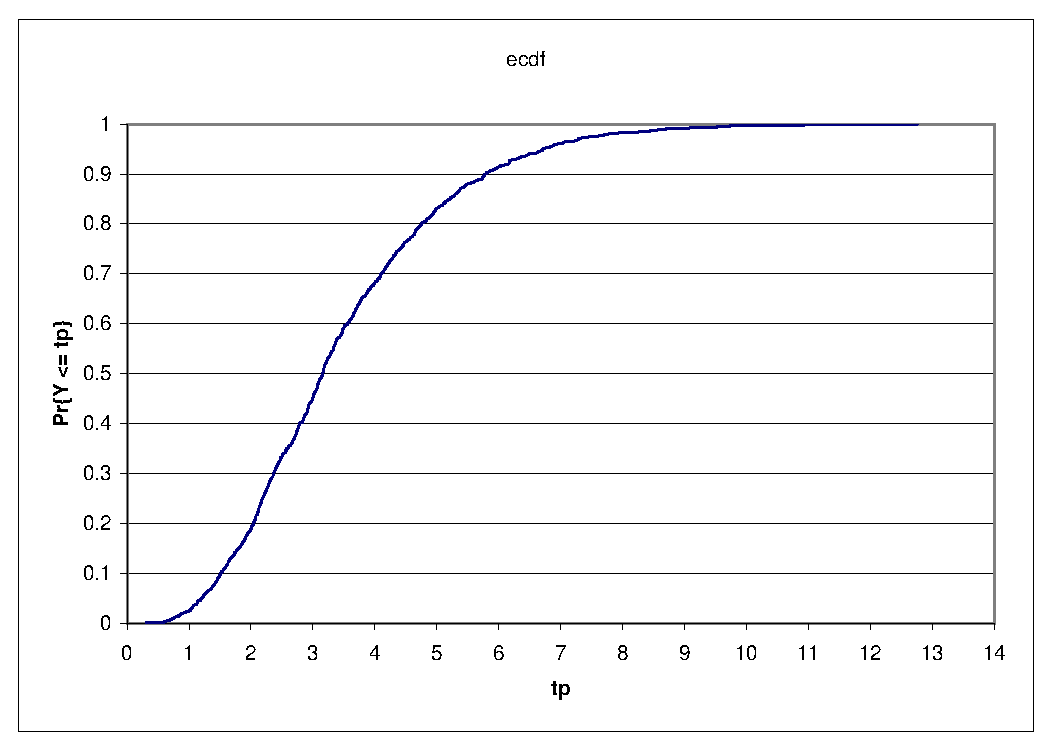
\includegraphics[width=4in]{figures/SANecdf}}
\caption{Empirical cdf of the project completion times.}
\label{fig:SANecdf}
\end{figure}

Notice (see Fig.~\ref{fig:san.de.mainsimulation}) that the simulation ends
when there are no additional activities remaining to be completed.

A difference between this implementation of the SAN simulation and the one in
Sect.~\ref{sec:san.max.sim} is that here we write out the actual
time the project completes on each replication. By doing so, we can
estimate $\Pr\{Y > t_p\}$ for any value of $t_p$ by sorting the data
and counting how many out of $1000$ replications were greater than
$t_p$. Figure~\ref{fig:SANecdf} shows the empirical cdf of the $1000$
project completion times, which is the simulation estimate
of Eq.~(3.12).%~(\ref{eq:san.analytic}).

\subsection{Issues and Extensions}
\label{sec:sim.san.issues}

\begin{enumerate}

\item In real projects there are not only activities, but also
limited and often shared resources that are needed to complete the
activities. Further, there may be specific resource allocation rules
when multiple activities contend for the same resource. How might
this be modeled in SimPy?

\item Time to complete the project is an important overall measure,
but at the planning stage it may be more important to discover which
activities or resources are the most critical to on-time completion
of the project. What additional output measures might be useful for
deciding which activities are ``critical?''

\end{enumerate}


\section{Simulating the Asian Option}
\label{sec:sim.asian}
\index{Asian option}


Here we consider estimating the value of an Asian option
\[
\nu = \E\left[ \mathrm{e}^{-rT} (\bar{X}(T) - K)^+ \right]
\]
as described in Sect.~(3.5),%\ref{sec:fe},
where the maturity is $T = 1$
year, the risk-free interest rate is $r = 0.05$ and the strike price
is $K = \$55$. The underlying asset has an initial value of $X(0) =
\$50$ and the volatility is $\sigma^2 = (0.3)^2$.  Recall that the
key quantity is
\[
\bar{X}(T) = \frac{1}{T}\int_0^T X(t)\, \D t
\]
the time average of a continuous-time, continuous-state geometric
Brownian motion
process which we cannot truly simulate on a digital computer.
\index{geometric Brownian motion}
Thus, we approximate it by dividing the
interval $[0, T]$ into $m$ steps of size $\Delta t =
T/m$ and using the discrete approximation
\[
\widehat{\bar{X}(T)} = \frac{1}{m}
\sum_{i=1}^m X(i \Delta t) .
\]
This makes simulation possible, since
\[
X(t_{i+1}) = X(t_i) \exp\left\{\left( r - \frac{1}{2}\sigma^2
\right)(t_{i+1}
- t_i) + \sigma\sqrt{t_{i+1} - t_i} \, Z_{i+1} \right\}
\]
for any increasing sequence of times $\{t_0, t_1, \ldots, t_m\}$,
where $Z_1, Z_2, \ldots, Z_m$ are i.i.d.\ $\mathrm{N}(0,1)$.

Figure~\ref{fig:asian.sim} is Python code that uses $m=32$ steps in
the approximation, and makes $10{,}000$ replications to estimate
$\nu$. Discrete-event structure would slow execution without any
obvious benefit, so a simple loop is used to advance time. The value
of the option from each replication is saved to a list for
post-simulation analysis.

The estimated value of $\nu$ is \$2.20 with a relative error of just over 2\%
(recall that the relative error is the standard error divided by the
mean). As the histogram in Fig.~\ref{fig:AsianHistogram} shows, the
option is frequently worthless (approximately 68\% of the time), but
the average payoff, conditional on the payoff being positive, is
approximately \$6.95.


\begin{figure}[tb]
\begin{center}
\begin{minipage}[t]{6in}\small
\verbatiminput{asianoption.py}
\end{minipage}
\end{center}
\caption{Python Simulation of the Asian option problem.}
\label{fig:asian.sim}
\end{figure}


\begin{figure}[tb]
\centerline{\includegraphics[width=4in]{figures/AsianHistogram}}
\caption{Histogram of the realized value of the Asian option from
10{,}000 replications.}
\label{fig:AsianHistogram}
\end{figure}

\section{Case Study: Service Center Simulation}
\label{sec:fax}

This section presents a simulation case based on a project provided by
a former student. While still relatively simple, it is more complex
than the previous stylized examples, and the answer is not known
without simulating. The purpose of this section is to illustrate how
one might attack simulation modeling and programming for a realistic
problem.

\begin{example}[Fax Center Staffing] \label{ex:fax}

A service center receives faxed orders throughout the day,
with the rate of arrival varying hour by hour. The arrivals are
modeled by a nonstationary Poisson process with the rates
shown in Table~\ref{tab:fax.arrivals}. \index{nonstationary Poisson
process}

\begin{table}[tb]
\caption{Arrival rate of faxes by hour.}
\label{tab:fax.arrivals}
\begin{center}
\begin{tabular}{lc}\hline
\multicolumn{1}{c}{Time}&Rate (faxes/minute) \\\hline
8 AM--9 AM & 4.37 \\
9 AM--10 AM & 6.24 \\
10 AM--11 AM & 5.29 \\
11 AM--12 PM & 2.97 \\
12 PM--1 PM & 2.03 \\
1 PM--2 PM & 2.79 \\
2 PM--3 PM & 2.36 \\
3 PM--4 PM & 1.04 \\\hline
\end{tabular}
\end{center}
\end{table}


A team of Entry Agents select faxes on a first-come-first-served basis
from the fax queue. Their time to process a fax is modeled as normally
distributed with mean $2.5$ minutes and standard deviation $1$ minute.
There are two possible outcomes after the Entry Agent finishes
processing a fax: either it was a simple fax and the work on it is
complete, or it was not simple and it needs to go to a Specialist for
further processing.  Over the course of a day, approximately 20\% of
the faxes require a Specialist.  The time for a Specialist to process
a fax is modeled as normally distributed with mean $4.0$ minutes and
standard deviation $1$ minute.

Minimizing the number of staff minimizes cost, but certain
service-level requirements much be achieved.  In particular, 96\% of
all simple faxes should be completed within $10$ minutes of their
arrival, while 80\% of faxes requiring a Specialist should also be
completed (by both the Entry Agent and the Specialist) within $10$
minutes of their arrival.

The service center is open from 8 AM to 4 PM daily, and it is possible
to change the staffing level at 12 PM. Thus, a staffing policy
consists of four numbers: the number of Entry Agents and Specialists
before noon, and the number of Entry Agents and Specialists after
noon.  Any fax that starts its processing before noon completes
processing by that same agent before the agent goes off duty; and
faxes in the queues at the end of the day are processed before the
agents leave work and therefore are not carried over to the next day.

\end{example}

\emph{The first step in building any simulation model is deciding
what question or questions that the model should answer.} Knowing the
questions helps identify the system performance measures that the
simulation needs to estimate, which in turn drives the scope and level
of detail in the simulation model.

The grand question for the service center is, what is the minimum
number of Entry Agents and Specialists needed for both time
periods to meet the service-level requirements?  Therefore, the
simulation must at least provide an estimate of the percentage of
faxes of each type entered within 10 minutes, given a specific staff
assignment.

Even when there seems to be a clear overall objective (minimize the
staff required to achieve the service-level requirement), we often
want to consider trade offs around that objective. For instance, if
meeting the requirement requires a staff that is so large that they
are frequently underutilized, or if employing the minimal staff means
that the Entry Agents or Specialists frequently have to work well past
the end of the day, then we might be willing to alter the
service requirement a bit.  Statistics on the number and the time
spent by faxes in queue, and when the last fax of each day is actually
completed, provide this information. Including additional measures
of system performance, beyond the most critical ones, makes the
simulation more useful.

Many discrete-event, stochastic simulations involve entities that
dynamically flow through some sort of queueing network where they
compete for resources. In such simulations, identifying the entities
and resources is a good place to start the model. For this service
center the faxes are clearly the dynamic entities, while the Entry
Agents and Specialists are resources. The fax machines themselves
might also be considered a resource, especially if they are heavily
utilized or if outgoing as well as incoming faxes use the same
machines. It turns out that for this service center there is a bank of
fax machines dedicated to incoming faxes, so it is reasonable to treat
the arrival of faxes as an unconstrained external arrival process.
This fact was not stated in the original description of the problem;
follow-up questions are often needed to fully understand the system of
interest.

Whenever there are scarce resources, queues may form. Queues are often
first-in-first-out, with one queue for each resource, as they are in
this service center. However, queues may have priorities,
and multiple queues may be served by the same resource, or a single
queue may feed multiple resources. Queueing behavior is often a
critical part of the model.

When the simulation involves entities flowing through a network of
queues, then there can be two types of arrivals: arrivals from outside
of the network and arrivals internal to the network. Outside
arrivals are like those we have already seen in the $M(t)/M/\infty$ and
$M/G/1$ examples.  Internal arrivals are departures from one queue
that become arrivals to others. How these are modeled depends largely
on whether the departure from one queue is an immediate arrival to the
next---in which case the departure and arrival events are effectively
the same thing---or whether there is some sort of transportation
delay---in which case the arrival to the next queue should be
scheduled as a distinct event.
For the service center the arrival of faxes to the Entry
Agents is an outside arrival process, while the 20\% of faxes that
require a Specialist are internal arrivals from the Entry Agents to
the Specialists.

Critical to experiment design is defining what constitutes a
replication. Replications should be independent and identically
distributed. Since the service center does not carry faxes over from
one day to the next, a ``day'' defines a replication. If faxes did
carry over, but all faxes are cleared weekly, then a replication might
be defined by a work week. However, if there is always significant
carry over from one day to the next, then a replication might have to
be defined arbitrarily.

The work day at the service center is eight hours;
however the staff does not leave until all faxes that arrive before 4
PM are processed. If we defined a replication to be exactly eight
hours then we could be fooled by a staffing policy that allows a large
queue of faxes to build up toward the end of the day, since the entry
of those faxes would not be included in our statistics. To model a
replication that ends when there is no additional work remaining, we
will cut off the fax arrivals at 4 PM and then end the simulation when
the event calendar is empty. This works because idle Entry Agents and
Specialists will always take a fax from their queue if one is
available.

Rather than walk through the SimPy code line by line, we will point
out some highlights to facilitate the reader's understanding of the
code.

Figure~\ref{fig:fax.global} shows the global declarations for the
service center simulation.


\begin{figure}[tbp]\small
\verbatiminput{faxcenter3.py}
\caption{Fax center program}
\label{fig:fax.global}
\end{figure}

\clearpage

The main program for the simulation is in Fig.~\ref{fig:fax.main}.
Of particular note are the two \Monitor\
statements defining \texttt{Regular10} and \texttt{Special10}. These
will be used to obtain the fraction of regular and special faxes that
are processed within the $10$-minute requirement by recording a $1$
for any fax that meets the requirement, and a $0$ otherwise. The mean
of these values is the desired fraction.

Also notice is the condition that ends the main simulation
loop:
\begin{center}
\texttt{self.simulate(until=F.maxTime)}
\end{center}

Because the simulation ends well after the arrivals cease, any faxes still in the queue will be completed prior to the end of the simulation.
When the event calendar is empty, then there are no additional faxes to
process, and no pending arrival of a fax. This condition will only
hold after 4 PM and once all remaining faxes have been entered.


Figure~\ref{fig:fax.agents} includes processes that generate faxes (\texttt{Source})
 and determine how they are routed to agents (\texttt{Fax}).
As faxes are routed, the simulation determines if they require special handling
after the regular agent is complete (\texttt{if (checkSpecial < F.pSpecial)}).
There are also two \Monitor\ present, \texttt{Regularwait} and \texttt{Specialistwait}
which record the total wait time for each fax that is completed.

\begin{verbatim}
            self.sim.Regularwait.observe(finished)
\end{verbatim}

Later, in the \texttt{reporting()}) function of the main program shown in Figure \ref{fig:fax.main},
this \Monitor\ will be used to both get the number of total faxes of this type, the number that waited less than 10 minutes before completing processing, and the fraction.

\begin{verbatim}
        regularcount = self.Regularwait.count()
        regular10min = sum([1.0 if waittime < 1./6 else 0
            for waittime in self.Regularwait.yseries()])
        fractionregular10min = regular10min/regularcount
\end{verbatim}

While collecting statistics in this fashion provides the most flexibility as it keeps
the wait time observations for future use, we could have instead recorded if
the wait time was less than 10 minutes.

\begin{verbatim}
	if finished < 1.0/6:  # 10 minutes
            self.sim.Regularwait.observe(1)
	else:
            self.sim.Regularwait.observe(0)
\end{verbatim}

Then we could have calculated the fraction by taking the sum of the observations divided by the number of observations.

\begin{verbatim}
        fractionregular10min = float(sum(self.Regularwait))/
            len(self.Regularwait)
\end{verbatim}

The \texttt{Fax.reporting()} then uses the \Monitor\ for wait time as well as the
monitors associated with the \texttt{agents} and \texttt{specialagents} resources.
The \texttt{actMon} monitors track how the resources are being used
while the \texttt{waitMon} monitors track the waiting queue for each monitor.
For resources, we tend to be interested in the time average value of the size of the queue
or the number of units of resource in use so the \texttt{agents.actMon.timeAverage()} function
returns the average utilization of the agents while \texttt{specialagents.waitMon.timeAverage()} function
returns the average number of special faxes in queue.

Ten replications of this simulation with a staffing policy of $15$
Entry Agents in the morning and $9$ in the afternoon, and $6$
Specialists in the morning and $3$ in the afternoon, gives $0.98 \pm
0.04$ for the fraction of regular faxes entered in $10$ minutes or
less, and $0.84 \pm 0.08$ for the special faxes. The ``$\pm$'' are
$95$\% confidence intervals. This policy appears to be close to the
requirements, although if we absolutely insist on $80$\% for the
special faxes then additional replications are needed to narrow the
confidence interval.


\begin{figure}[tbp]\small
REMOVED
\caption{Processes for arriving agents.}
\label{fig:fax.agents}
\end{figure}


\begin{figure}[tbp]\small
REMOVED
\caption{Processes handling changes over time.}
\label{fig:fax.shifts}
\end{figure}

\clearpage


\begin{figure}[tbp]
REMOVED
\caption{Parameters for service center simulation.}
\label{fig:fax.initial}
\end{figure}

\subsection{Issues and Extensions}
\label{sec:sim.fax.issues}

\begin{enumerate}

\item There are many similarities between the programming for this
simulation and the event-based simulation of the $M/G/1$ queue.



\item The fax entry times were modeled as being normally distributed.
However, the normal distribution admits negative values, which
certainly does not make sense. What should be done about this?
Consider mapping negative values to 0, or generating a new value
whenever a negative value occurs. Which is more likely to be realistic
and why?

\end{enumerate}

\section*{Exercises}
\addcontentsline{toc}{section}{Exercises}

\begin{enumerate}

\item For the hospital problem, simulate the current system in which the
receptionist's service time is well modeled as having an Erlang-$4$
distribution with mean $0.6$ minutes. Compare the waiting time to the
proposed electronic kiosk alternative.

\item Simulate an $M(t)/G/\infty$ queue where $G$ corresponds to an
Erlang distribution with fixed mean but try different numbers of
phases. That is, keep the mean service time fixed but change the
variability. Is the expected number if queue sensitive to the
variance in the service time?

\item Modify the SAN simulation to allow each activity to have a
different mean time to complete (currently they all have mean time
$1$). Use a Collection to hold these mean times.

\item Try the following numbers of steps for approximating the value
of the Asian option to see how sensitive the value is to the step
size: $m=8, 16, 32, 64, 128$.

\item In the simulation of the Asian option, the sample mean of
10{,}000 replications was $2.198270479$, and the standard deviation
was $4.770393202$. Approximately how many replications would it take
to decrease the relative error to less than 1\%?

\item For the service center, increase the number of replications
until you can be confident that that suggested policy does or does not
achieve the $80$\% entry in less than $10$ minutes requirement for
special faxes.

\item For the service center, find the minimum staffing policy (in
terms of total number of staff) that achieves the service-level
requirement.  Examine the other statistics generated by the simulation
to make sure you are satisfied with this policy.

\item For the service center, suppose that Specialists earn twice as
much as Entry Agents.  Find the minimum cost staffing policy that
achieves the service-level requirement. Examine the other statistics
generated by the simulation to make sure you are satisfied with this
policy.

\item For the service center, suppose that the staffing level can
change hourly, but once an Agent or Specialist comes on duty they
must work for four hours. Find the minimum staffing policy (in
terms of total number of staff) that achieves the service-level
requirement.

\item For the service center, pick a staffing policy that fails to
achieve the service level requirements by $20$\% or more. Rerun the
simulation with a replication being defined as exactly 8 hours, but do
not carry waiting faxes over to the next day. How much do the
statistics differ using the two different ways to end a replication?


\item The function \verb+NSPP_Fax+ is listed below. This function
implements the thinning method described in
Sect.~\ref{sec:sim.mminf} for a nonstationary Poisson process with
piecewise-constant rate function. Study it and describe how it works.
\index{nonstationary Poisson process} \index{thinning}

\small
\begin{verbatim}
def NSPP_Fax(arrivalrate, MaxRate, NPeriods, periodlength, stream):
    '''  Non-stationary Poisson Process

    This function generates interarrival times from a NSPP with
    piecewise constant arrival rate over a fixed time of NPeriod time units

    arrivalrate - Array of arrival rates over a common length period
    MaxRate - The maximum value of ARate
    NPeriods - Number of time periods in ARate
    periodlength - time units between (possible) changes in arrival rate
    '''
    random.seed(stream)
    pthinning = [(1-hourlyrate/MaxRate) for hourlyrate in arrivalrate]
    t = 0.0
    arrivaltimes = []
    totaltime = NPeriods * periodlength
    while t < totaltime:
        deltat = random.expovariate(MaxRate)
        t = t + deltat
        if t < totaltime:
            pthin = pthinning[int(floor(t/periodlength))]
            uthin = random.random()
            if uthin > pthin:
                arrivaltimes.append(float(t)) # add arrival since not thinned
    return arrivaltimes
\end{verbatim} \normalsize

\item  Beginning with the event-based $M/G/1$ simulation,
implement the changes necessary to make it an $M/G/s$ simulation (a
single queue with any number of servers). Keeping $\lambda = 1$ and
$\tau/s = 0.8$, simulate $s=1,2,3$ servers and compare the results.
What you are doing is comparing queues with the same service capacity,
but with $1$ fast server as compared to two or more slower servers.
State clearly what you observe.

\item  Modify the SimPy event-based simulation of the $M/G/1$
queue to simulate an M/G/1/$c$ retrial queue. This means that customers
who arrive to find $c$ customers in the system (including the customer
in service) leave immediately, but arrive again after an exponentially
distributed amount of time with mean \texttt{MeanTR}.  Hint: The
existence of retrial customers should not affect the arrival process for
first-time arrivals.

\item  This problem assumes a more advanced background in
stochastic processes. In the simulation of the $M(t)/M/\infty$ queue
there could be a very large number of events on the event calendar: one
``Arrival'' and one ``Departure'' for \textit{each} car currently in the
garage. However, properties of the exponential distribution can reduce
this to no more than two events.  Let $\beta = 1/\tau$ be the departure
rate for a car (recall that $\tau$ is the mean parking time). If at any
time we observe that there are $N$ car in the garage (no matter how long
they have been there), then the time until the first of these cars
departs is exponentially distributed with mean $1/(N\beta)$. Use this
insight to build an $M(t)/M/\infty$ simulation with at most two pending
events, next arrival and next departure. Hint: Whenever an arrival
occurs the distribution of the time until the next departure changes, so
the scheduled next departure time must again be generated.


\item  The phone desk for a small office is staffed from 8 AM
to 4 PM by a single operator. Calls arrive according to a Poisson
process with rate 6 per hour, and the time to serve a call is uniformly
distributed between 5 and 12 minutes.  Callers who find the operator
busy are placed on hold, if there is space available, otherwise they
receive a busy signal and the call is considered ``lost.'' In addition,
10\% of callers who do not immediately get the operator decide to hang
up rather than go on hold; they are not considered lost, since it was
their choice. Because the hold queue occupies resources, the company
would like to know the smallest capacity (number of callers) for the
hold queue that keeps the daily fraction of lost calls under 5\%. In
addition, they would like to know the long-run utilization of the
operator to make sure he or she will not be too busy.  Use SimPy to
simulate this system and find the required capacity for the hold queue.
Model the callers as a Process and the operator as a \textbf{Resource}.
Use the functions \texttt{random.expovariate} and \texttt{random.uniform} for random-variate
generation.  Estimate the fraction of calls
lost (record a 0 for calls not lost, a 1 for those that are lost so that
the sample mean is the fraction lost). Use the statistics collected by class
Resource to estimate the utilization.


\item \label{ex:smp} Software Made Personal (SMP)
customizes software products in two areas: financial tracking and
contact management.  They currently have a customer support call
center that handles technical questions for owners of their software
from the hours of 8 AM to 4 PM Eastern Time.

When a customer calls they the first listen to a recording that asks
them to select among the product lines; historically 59\% are financial
products and 41\% contact management products. The number of customers
who can be connected (talking to an agent or on hold) at any one time is
essentially unlimited.  Each product line has its own agents. If an
appropriate agent is available then the call is immediately routed to
the agent; if an appropriate agent is not available, then the caller is
placed in a hold queue (and listens to a combination of music and ads).
SMP has observed that hang ups very rarely happen.

SMP is hoping to reduce the total number of agents they need by
cross-training agents so that they can answer calls for any product
line.  Since the agents will not be experts across all products, this
is expected to increase the time to process a call by about 5\%.  The
question that SMP has asked you to answer is how many cross-trained
agents are needed to provide service at the same level as the current
system.

Incoming calls can be modeled as a Poisson arrival process with a rate
of $60$ per hour.  The mean time required for an agent to answer a
question is $5$ minutes, with the actual time being Erlang-$2$ for
financial calls, and Erlang-$3$ for contact management calls.  The
current assignment of agents is $4$ for financial and $3$ for contact
management.  Simulate the system to find out how many agents are
needed to deliver the same level of service in the cross-trained system
as in the current system.
\end{enumerate}


\begin{thebibliography}{99}

\bibitem{SimPy2016} Team SimPy, {\em SimPy Simulation Package},   \url{https://simpy.readthedocs.io/en/latest/}, 2016.
\bibitem{Scipy2001} Eric Jones, Travis Oliphant, Pearu Peterson, and others, {\em SciPy: Open Source Scientific Tools for Python},  \url{http://www.scipy.org/}, 2001.
\bibitem{Law2007} Averill M. Law, {\em Simulation Modeling \& Analysis}, 4th ed., McGraw-Hill: New York, NY, 
2007.
\bibitem{Nelson2013} Barry Nelson, {\em Foundations and Methods for Stochastic Simulation|}, Springer: Boston, MA, 2013.
\end{thebibliography}

\end{document}
